\label{chap:wikt}
Rozdział ten stanowi charakterystykę Wikisłownika --- sieciowego słownika opartego na oprogramowaniu MediaWiki. Wikisłownik jest jednym z~największych i~najpopularniejszych słowników dostępnych w~polskim internecie. W~kolejnych podrozdziałach projekt ten został opisany na różnych poziomach szczegółowości. Omówiono zarówno oprogramowanie, na jakim bazuje słownik, jak i~swego rodzaju ,,ekosystem'', w~którym znajduje on swoje miejsce.

\section{Projekty Fundacji Wikimedia}
Podmiotem odpowiedzialnym m.in. za rozwój Wikisłownika jest Wikimedia Foundation Inc. (opisywana dalej jako \emph{Fundacja}) --- organizacja non\dywiz{}profit mająca siedzibę w~San Francisco w~Stanach Zjednoczonych, istniejąca od 2003 roku. Jak informuje strona internetowa polskiego partnera Fundacji, Stowarzyszenia Wikimedia Polska, \emph{celem fundacji jest sprzyjanie tworzeniu i~rozwojowi projektów o~otwartej treści opartych na technologii WikiWiki oraz dostarczanie społeczności internetowej pełnej zawartości wymienionych projektów za darmo i~bez zamieszczania reklam}~\cite{wm:pl}. Doskonale znaną, sztandarową inicjatywą Fundacji jest Wikipedia (\url{http://www.wikipedia.org}) --- największa obecnie encyklopedia internetowa, dostępna w~281~językach (stan z~sierpnia 2011 roku) i~zawierająca ponad 19~milionów haseł, w~tym ponad 3,7~miliona w~największej, angielskojęzycznej\footnote{Oficjalnie w~projektach Fundacji używane są określenia typu \emph{angielskojęzyczny}, \emph{polskojęzyczny}. Choć w~przypadku wersji polskojęzycznej znakomita większość uczestników projektów pochodzi z~Polski, nie jest to regułą dla innych edycji. W~dalszej części pracy przyjęto następujące uproszczenie: określenia typu \emph{polska Wikipedia}, \emph{angielski Wikisłownik} traktowane są jako tożsame z~określeniami używającymi sformułowań z~cząstką \emph{-języczny}.} edycji \cite{wiki:list}. Mimo częstej krytyki tego przedsięwzięcia faktem jest, że Wikipedia jest miejscem, z~którego miliony osób korzystają, by pozyskać informacje z~najróżniejszych dziedzin. Obecny stan rzeczy możliwy jest dzięki pracy wielkiej liczby wolontariuszy tworzących artykuły bez wynagrodzenia.

\begin{illustration}
	\fbox{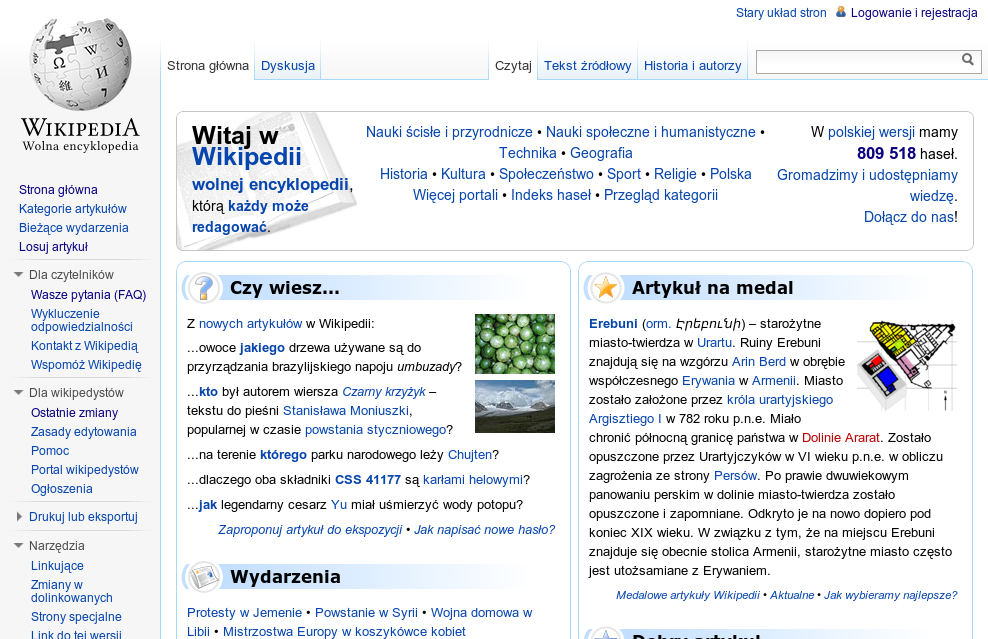
\includegraphics{plwikipedia}}
	\caption{Polska edycja Wikipedii}
\end{illustration}

Wikipedia jest najbardziej znanym, ale nie jedynym projektem pod opieką Fundacji. Pozostałe to tzw. ,,projekty siostrzane'', w~szczególny sposób uwzględniane również przy tworzeniu haseł w~encyklopedii. Oto lista wspieranych przez Fundację wielojęzycznych inicjatyw~\cite{wm:main}:
\begin{itemize}
	\item Wikisłownik (ang. \emph{Wiktionary}) --- wielojęzyczny słownik internetowy, będący głównym przedmiotem niniejszej pracy,
	\item Wikicytaty (ang. \emph{Wikiquotes}) --- zbiór cytatów autorstwa znanych osób, z~filmów i~książek, przysłów i~porzekadeł,
	\item Wikibooks --- serwis z~,,otwartymi'' (opartymi na wolnej licencji) podręcznikami,
	\item Wikiźródła (ang. \emph{Wikisource}) --- zbiór dokumentów źródłowych w~wersjach oryginalnych i~tłumaczonych, nieograniczonych prawem autorskim,
	\item Wikinews --- otwarty serwis informacyjny,
	\item Wikiversity --- materiały edukacyjne i~naukowe,
	\item Wikispecies --- katalog gatunków organizmów żywych,
	\item MediaWiki --- nadzór nad tworzeniem i~rozpowszechnianiem oprogramowania MediaWiki (p.~podrozdział~\ref{sec:mw}),
	\item Meta\dywiz{}Wiki --- projekt ułatwiający koordynację wszystkich pozostałych.
	\item Wikimedia Commons --- repozytorium mediów (zdjęć, grafik, filmów) dostępnych na wolnej licencji, z~którego korzystają pozostałe projekty Wikimedia,
	\item Wikimedia Incubator --- metaprojekt umożliwiający tworzenie nowych inicjatyw wspieranych przez Fundację.
\end{itemize}
Wszystkie projekty łączy sposób ich powstawania --- możliwość edycji dostępna jest praktycznie dla każdego internauty. Nie dotyczy to co~prawda kilku krajów, w~których projekty Fundacji zablokowane są w~ramach cenzury internetu, jednak ogromna większość osób dysponujących łączem internetowym ma szansę stać się jednymi spośród współautorów haseł.

Drugą cechą wspólną są wolne licencje, na których udostępniana jest zawartość wszystkich serwisów. Po reformie w~czerwcu 2009~roku treść Wikipedii i~projektów siostrzanych dostępna jest nie tylko na licencji GNU FDL (Free Documentation License)~1.2, ale także na kompatybilnej z~nią CC\dywiz{}BY\dywiz{}SA 3.0 (Creative Commons Attribution\dywiz{}ShareAlike / Uznanie Autorstwa --- Na Tych Samych Warunkach)~\cite{wiki:license}. Oznacza to, że można ją dowolnie wykorzystywać we~własnych dziełach pod warunkiem podania oryginalnych autorów i~zachowania pierwotnej licencji.

\section{Oprogramowanie MediaWiki}
\label{sec:mw}
Sama działalność wolontariacka redaktorów projektów Wikimedia nie wystarczyłaby do stworzenia serwisów internetowych o~obecnych kształtach. Konieczne jest oczywiście również zapewnienie oprogramowania, które umożliwi płynną współpracę przy tworzeniu haseł. Tym oprogramowaniem jest wolna platforma MediaWiki tworzona zgodnie z~zasadami \emph{open source}. System MediaWiki napisany jest w~języku PHP i~obsługuje kilka popularnych baz danych (w~przypadku projektów Wikimedia jest to MySQL). Dla inicjatyw Wikimedia stanowi szkielet programistyczny od samego ich początku, a~od 2002~roku stale się rozwija. W~czerwcu 2011~roku wersją używaną w~projektach było MediaWiki~1.17.

System MediaWiki używany jest nie tylko w~projektach wspieranych przez Fundację, ale także w~tysiącach innych, mniejszych lub większych, co jest możliwe dzięki wysokiemu stopniowi konfigurowalności i~dużej liczbie dostępnych rozszerzeń. Są to w~dużej mierze serwisy o~podobnym charakterze, umożliwiające swobodną wymianę informacji na dowolny temat. MediaWiki bywa także używane w~firmowych intranetach i~wszędzie tam, gdzie zachodzi potrzeba udostępnienia materiałów do edycji dużej liczbie użytkowników.

\subsection{Edytowanie i~wikitekst}
Strony w~projektach opartych na platformie MediaWiki na~ogół nie mogą być czystym tekstem, pozbawionym formatowania. Przykładowo hasła w~encyklopedii muszą zachowywać określoną strukturę --- występuje więc podział na sekcje, ilustracje, różne rodzaje formatowania (kursywa, wytłuszczenie), przypisy czy powtarzalne fragmenty. Szczególnie istotnym elementem są linki pomiędzy poszczególnymi artykułami, wyróżniające projekty Fundacji na tle ich papierowych, ale też elektronicznych konkurentów. Odnośniki pozwalają błyskawicznie przemieszczać się między hasłami, by w~ten sposób uzyskiwać kolejne informacje wspomagające przyswajanie wiedzy.

Linki i~formatowanie na stronach internetowych tworzone są za pomocą elementów języka HTML lub XHTML. O~ile języki te są proste w~obsłudze dla specjalisty informatyka, to laik nie jest w~stanie tworzyć za ich pomocą stron bez uprzedniego dłuższego przygotowania. Aby umożliwić bezproblemową edycję stron internetowych osobom bez wykształcenia informatycznego, programiści MediaWiki zaprojektowali tzw. wikitekst~\cite{mw:help} --- uproszczony język opisu stron, pozwalający na realizację wymienionych elementów. Porównanie niektórych z~nich znajduje się w~tabeli~\ref{tab:html-wiki}.

\begin{table}[h]
\begin{center}
\footnotesize{
	\begin{tabularx}{\textwidth}{ lXX }
		\toprule & \textbf{Wikitekst} & \textbf{XHTML} \\
		\toprule Kursywa & \texttt{''Tekst''} & \texttt{<em>Tekst</em>} \\
		\midrule Wytłuszczenie & \texttt{'''Tekst'''} & \texttt{<strong>Tekst</strong>} \\
		\midrule Nagłówek & \texttt{== Nagłówek ==} & \texttt{<h2>Nagłówek</h2>} \\
		 & \texttt{=== Nagłówek ===} & \texttt{<h3>Nagłówek</h3>} \\
		\midrule Odnośnik wewnętrzny & \texttt{[[Strona]]} & \texttt{<a href="/wiki/Strona">Strona</a>} \\
		 & \texttt{[[Strona|strony]]} & \texttt{<a href="/wiki/Strona">strony</a>} \\
		\midrule Odnośnik zewnętrzny & \texttt{[http://www.google.com Google]}
		 & \texttt{<a href="http://www.google.com">\newline Google</a>} \\
		\midrule Obraz & \texttt{[[Plik:Przykład.png|thumb|Podpis]]}
		 & \texttt{<img src=".../Przykład.png"/><br/>\newline <div class="caption">Podpis</div>} \\
		\midrule Podział na akapity & \texttt{Pierwszy akapit \newline \newline Drugi akapit}
		 & \texttt{<p>Pierwszy akapit</p>\newline <p>Drugi akapit</p>} \\
		\midrule Lista nienumerowana & \texttt{* Element\newline * Element\newline * Element}
		 & \texttt{<ul>\newline <li>Element</li>\newline <li>Element</li>\newline <li>Element</li>\newline </ul>}\\
		\midrule Lista numerowana & \texttt{\# Element\newline \# Element\newline \# Element}
		 & \texttt{<ol>\newline <li>Element</li>\newline <li>Element</li>\newline <li>Element</li>\newline </ol>}\\
		\bottomrule
	\end{tabularx}
}
\caption{Porównanie HTML i wikitekstu}
\label{tab:html-wiki}
\end{center}
\end{table}

Łatwo można zauważyć, że używanie wikitekstu jest o~wiele prostsze niż nauka języka XHTML. Jeśli zachodzi potrzeba zaawansowanego formatowania, możliwe jest także użycie znaczników XHTML. W~przypadku standardowego formatowania jest to jednak niewskazane ze względu na dobro niedoświadczonych edytorów.

Bardzo istotnym elementem wikitekstu są szablony --- predefiniowane fragmenty kodu z~opcjonalnymi parametrami. Szablony można uznać za odpowiednik procedur/funkcji w~językach programowania. W~projektach opartych na MediaWiki szablony pełnią przede wszystkim dwie główne funkcje:
\begin{itemize}
	\item upraszczają kod --- pozwalają np. na zastąpienie skomplikowanego kodu XHTML (a~także jeszcze bardziej złożonych funkcji parsera MediaWiki) krótkim wywołaniem szablonu,
	\item standaryzują strony --- często wykorzystywane fragmenty wywoływane są zawsze w~dokładnie ten sam sposób.
\end{itemize}
We~wszystkich większych projektach Fundacji szablony są bardzo często wykorzystywane. Przy tym stanowią duże ułatwienie dla technicznie zaawansowanych autorów, którzy wspomagają się przy tworzeniu haseł dodatkowymi technologiami. Na używaniu szablonów korzystają przede wszystkim boty, czyli programy dokonujące edycji samodzielnie po uprzednim przygotowaniu lub pod stałą opieką programisty. W~większości projektów przyjęte jest, że każdy bot ma własne konto użytkownika, nie używa natomiast konta swojego ,,właściciela''. Dzięki botom możliwe jest np. masowe tworzenie haseł w~Wikipedii na ściśle określony temat, jeśli istnieje dobre źródło w~formie czytelnej dla komputera (takich jak opisy asteroid czy wszystkich miejscowości lub jednostek administracyjnych w~danym kraju). Innym ich zastosowaniem jest automatycznie uzupełnianie tzw. interwiki --- czyli odnośników pomiędzy poszczególnymi wersjami językowymi tego samego hasła.

Szablony mogą być wykorzystywane w~prosty sposób nawet przez początkujących użytkowników --- aby wywołać szablon, wystarczy wpisać jego nazwę
 pomiędzy podwójnymi nawiasami klamrowymi (\kod@{{Nazwa szablonu}}@ lub \kod@{{Nazwa szablonu|parametr=abc}}@). W~polskim Wikisłowniku szablony pełnią szczególną rolę --- pomysł na niniejszą pracę zrodził się m.in. dzięki ich szerokiemu zastosowaniu w~projekcie. Szczegóły tego zagadnienia zostaną przedstawione w~podrozdziale~\ref{sec:plwikt}.

\section{Wiktionary --- Wikisłownik}
\begin{illustration}
	\fbox{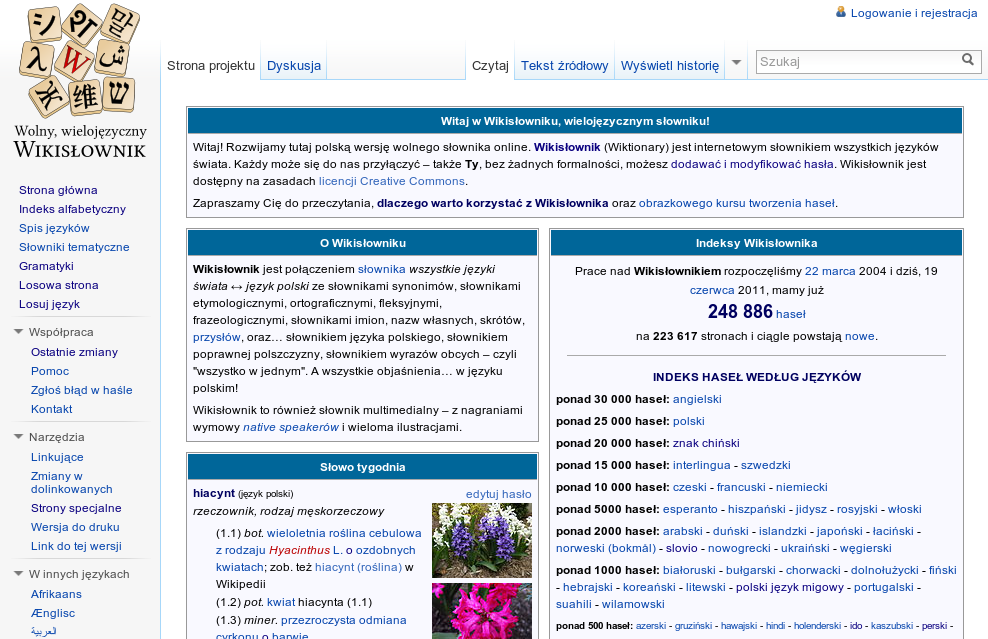
\includegraphics{plwikt}}
	\caption{Polska edycja Wikisłownika}
\end{illustration}
Jednym z~największych projektów siostrzanych Wikipedii jest Wikisłownik, w~wersji angielskiej (i~wielu innych) noszący nazwę \emph{Wiktionary} (\url{http://www.wiktionary.org}). Ten słownik internetowy nie rozwinął się jeszcze tak prężnie jak encyklopedia, zwłaszcza jeśli chodzi o~polską edycję. Jest dziś jednak jednym z~największych słowników w~sieci, a~w~pewnych zastosowaniach stanowi najlepszy wybór. Dużą zaletą Wikisłownika jest jego wielojęzyczność --- w~tym samym serwisie znaleźć można hasła w~ponad~250~językach. W~przypadku niektórych z~nich jest to praktycznie jedyny słownik internetowy lub nawet jedyny dostępny słownik w~ogóle. Przykładem może być polski Wikisłownik, który zawiera prawdopodobnie jedyny polski słownik języka hawajskiego czy największe słowniki języków suahili i~jidysz~\cite{wikt:dlaczego}.

Wspomniane zostało zastosowanie szablonów do standaryzacji kodu źródłowego i~struktury haseł. Trzeba jednak zaznaczyć, że dotyczy to wyłącznie haseł w~obrębie jednej wersji językowej Wikisłownika, są one bowiem niezależne od siebie i~od Fundacji. Wspólne dla wszystkich edycji jest jedynie oprogramowanie MediaWiki i~umiejscowienie na serwerach Fundacji pod adresem \kod|xxx.wiktionary.org|, gdzie zamiast \kod|xxx| wstawiany jest dwu- lub trzyliterowy skrót ISO języka (np. \url{pl.wiktionary.org} = język polski, \url{de.wiktionary.org} = język niemiecki, \url{sq.wiktionary.org} = język albański, \url{csb.wiktionary.org} = język kaszubski). Wszystkie kwestie organizacyjne w~obrębie wersji językowej ustalane są przez internetową społeczność w~ramach dyskusji i~głosowań. Głosowania służą także wyborowi administratorów projektu, czyli użytkowników mających dodatkowe uprawnienia, spośród których najważniejsze to usuwanie i~zabezpieczanie haseł oraz blokowanie użytkowników działających na szkodę projektu. W~lipcu 2011~roku w~angielskim Wikisłowniku działało aktywnie 76~administratorów~\cite{enwikt:admin}, zaś w~polskim --- 14~\cite{wikt:admin}. Dla porównania Wikipedia w~języku angielskim miała w~tym samym czasie 1541~administratorów (niekoniecznie aktywnych), wersja polska natomiast 163~\cite{wiki:admin}.

Podobnie jak w~przypadku Wikipedii, hasła w~poszczególnych wersjach językowych Wikisłownika są łączone poprzez odnośniki interwiki, znajdujące się na dole lewego menu w~większości haseł. W~stosunku do encyklopedii występuje znacząca różnica w~sposobie funkcjonowania tych linków. Wikipedia poprzez interwiki łączy artykuły na ten sam temat, często różniące się tytułem (polski artykuł \emph{Kot domowy} odsyła do angielskiego \emph{Cat} czy niemieckiego \emph{Hauskatze}). W~Wikisłowniku mechanizm interwiki łączy zaś strony o~tym samym tytule, niezależnie od ich zawartości. Polskie hasło \emph{kot} zawiera więc łącza do haseł o~tytule \emph{kot} w~innych językach, które mogą, ale nie muszą zawierać m.in. objaśnienia polskiego znaczenia tego słowa. Z~tego względu łatwo jest odnaleźć brakujące informacje o~wybranym słowie w~danym języku, jeśli skorzysta się z~kilku edycji językowych Wikisłownika. Natomiast tłumaczenia tytułu hasła na inne języki znajdują się bezpośrednio w~treści artykułu, w~miejscu przeznaczonym dla takich informacji.

Choć poszczególne wersje Wikisłownika różnią się między sobą, wspólna jest struktura hasła na najogólniejszym poziomie. Każde hasło jest podzielone na sekcje nagłówkami (p.~tabela~\ref{tab:html-wiki}), podobnie jak w~innych projektach Fundacji. W~przypadku słownika sposób podziału artykułu został jasno sprecyzowany i~jest wspólny dla wszystkich edycji. W~każdej z~sekcji objaśniono znaczenie tytułowego hasła w~innym języku. Przykładowo hasło \emph{nie} w~większości wersji językowych ma sekcje objaśniające znaczenie m.in. w~języku polskim oraz języku niemieckim (\emph{nigdy}). Właśnie ta ogólna cecha struktury haseł pozwala na częściową automatyzację niektórych często wykonywanych w~trakcie edycji czynności.

Aplikacja opisana w~niniejszej pracy przeznaczona jest dla polskiej edycji Wikisłownika. Konieczne jest zatem scharakteryzowanie specyfiki tego projektu (p.~podrozdział~\ref{sec:plwikt}). Ze~względu na odmienność poszczególnych wersji językowych prawdopodobnie w~innych nie będzie można wykorzystać wykorzystać aplikacji. Z~pewnością może ona być dla nich jednak bardzo przydatna --- duża część funkcji przez nią realizowanych może być używana niezależnie od specyfiki danej wersji, a~budowa aplikacji pozwoli na ich wyodrębnienie.

\section{Polska edycja Wikisłownika}
\label{sec:plwikt}
Wikisłownik w~języku polskim powstał 22~marca 2004~r.~\cite{wikt:home} i~jest dziś jedną z~najlepiej rozwiniętych edycji. Jeśli chodzi o~liczbę haseł, polska wersja zawiera ich ponad 230~000 i~znajduje się na 8.~miejscu (pierwsze trzy miejsca zajmują z~dużą przewagą edycje angielska, francuska i~chińska). Warto zwrócić jednak uwagę, że liczba artykułów nie musi odzwierciedlać ogólnego poziomu rozwoju danej edycji, a~przynajmniej w~o~wiele mniejszym stopniu niż w~Wikipedii. Automatyczne importowanie haseł słownikowych z~innych źródeł jest prostsze niż w~przypadku wpisów do~encyklopedii, a~hasła takie oczywiście nie wyróżniają się pozytywnie, jeśli wziąć pod lupę ich jakość. Wydaje się, że lepszym wskaźnikiem rozwoju są np. liczby aktywnych użytkowników lub administratorów. Tutaj polski Wikisłownik okazuje się wielokrotnie lepszy niż edycje litewska czy malajska, górujące nad nim pod względem liczby haseł~\cite{wikt:list}.

Poniżej opisana została dokładnie struktura haseł w~polskim Wikisłowniku. Społeczność tego projektu scharakteryzowano natomiast w~podrozdziale~\ref{sec:plsoc}.

\subsection{Struktura hasła}
\label{wikt:structure}
Jak wspomniano, wspólny dla wszystkich wersji językowych Wikisłownika jest podział na sekcje, odpowiadające poszczególnym językom. Polska edycja Wikisłownika jest bardzo dobrze ustrukturyzowana w~dalszym zakresie, co niekoniecznie jest regułą dla pozostałych edycji. Wynikiem tego jest jednolity wygląd hasła, który otrzymuje czytelnik, oraz jednolity kod widziany przez redaktora. Przykładowy artykuł z~jedną sekcją językową znajduje się na ilustracji~\ref{fig:plhaslo}.

\begin{illustration}
	\fbox{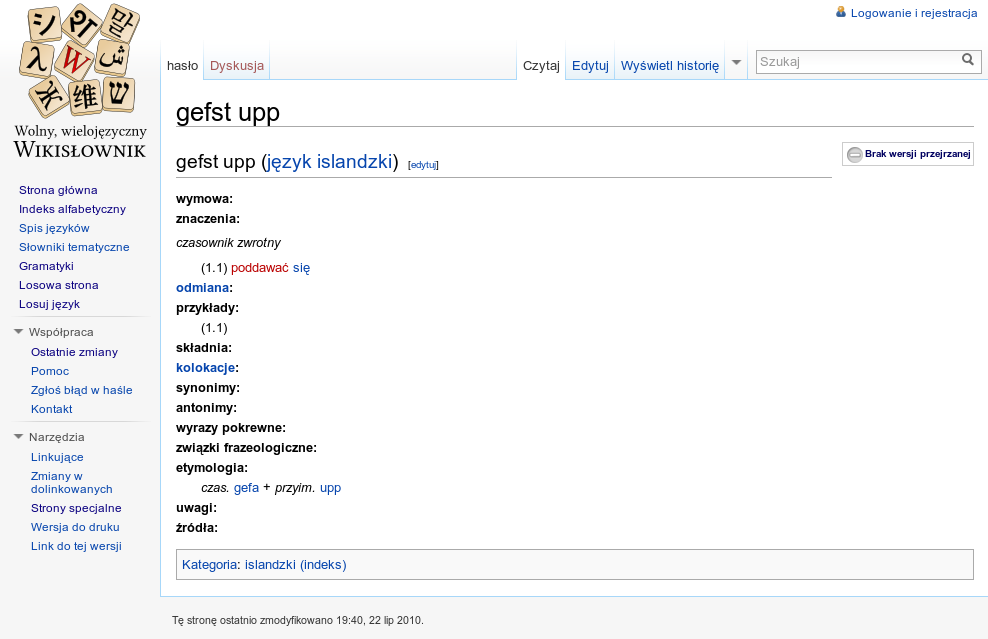
\includegraphics{plwikt-art}}
	\caption
		[Hasło w~polskim Wikisłowniku]
		{Hasło \emph{gefst upp} w~polskim Wikisłowniku (\protect\url{http://pl.wiktionary.org/wiki/gefst_upp})}
	\label{fig:plhaslo}
\end{illustration}

Na zrzucie ekranu widoczny jest układ sekcji typowy dla polskiego projektu. Z~małymi wyjątkami sekcje danego języka wyglądają tak samo we~wszystkich hasłach. To oznacza, że także w~innych opisanych wyrazach języka islandzkiego znaleźć można elementy: wymowa, znaczenia, odmiana, przykłady, składnia, kolokacje, synonimy, antonimy, wyrazy pokrewne, związki frazeologiczne, etymologia, uwagi, źródła. W~rzeczywistości jest to układ typowy dla znakomitej większości występujących w~Wikisłowniku języków~\cite{wikt:zasady}. Odstępstwa od tego szkieletu hasła są niewielkie i~zostaną przedstawione poniżej.

Ilustracja~\ref{fig:plhaslo-edit} przedstawia wygląd przykładowej strony po przejściu do trybu edycji, dostępnego dla każdego użytkownika (bez konieczności logowania). Widok ten prezentuje źródłowy wikikod hasła, dodatkowo edytor ma kilka ikon ułatwiających wstawianie często używanych elementów. W~kodzie tym widoczne są szablony definiujące tytuły poszczególnych elementów sekcji (nazywanych dalej \emph{podsekcjami}). Podział na sekcje i~podsekcje jest dość prosty do wykonania za pomocą programu komputerowego i~już sama ta procedura pozwala na znaczne zwiększenie przejrzystości w~nowym edytorze, opisanym w~rozdziale~\ref{chap:impl}.

\begin{illustration}
	\fbox{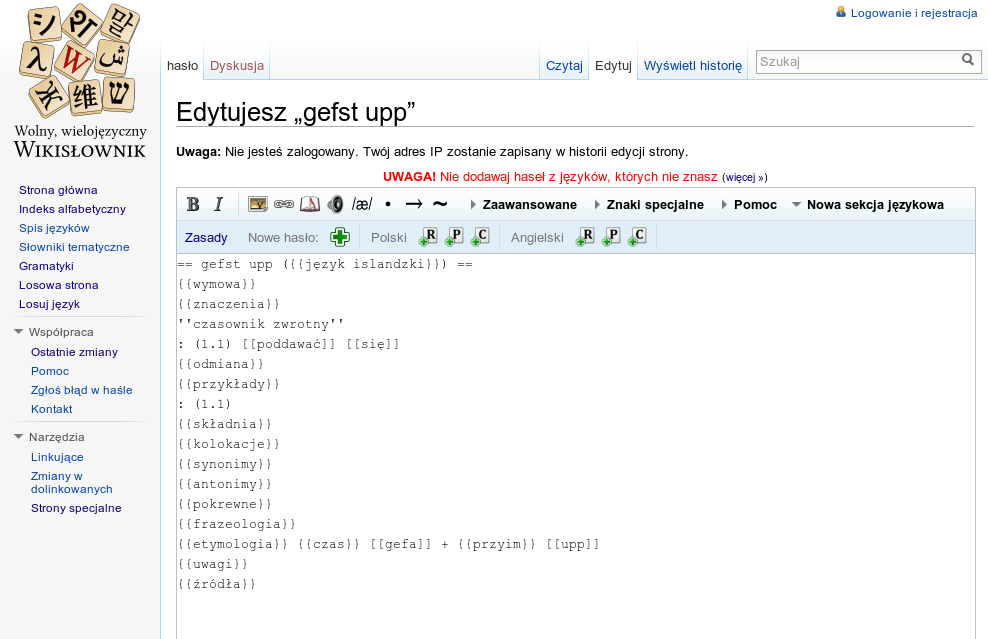
\includegraphics{plwikt-edit}}
	\caption
		[Edycja hasła w~polskim Wikisłowniku]
		{Edycja hasła \emph{gefst upp} w~polskim Wikisłowniku (\protect\url{http://pl.wiktionary.org/w/index.php?title=gefst_upp&action=edit})}
	\label{fig:plhaslo-edit}
\end{illustration}

Każda z~podsekcji w~hasłach ma ściśle określoną funkcję, dzięki której polski Wikisłownik jest jednolity. W~dodatku~\ref{wikt:subsections} omówione zostały wszystkie podsekcje występujące w~artykułach, w~jedynej uznanej za poprawną kolejności. Duża ich część pojawia się jedynie w~niektórych językach, dlatego choć lista podsekcji jest dość długa, to każde hasło będzie miało ich o~wiele mniej. Szablony podsekcji zebrane są na stronie \url{http://pl.wiktionary.org/wiki/Kategoria:Szablony_szablonów_haseł}. Szczególną uwagę należy zwrócić na takie podsekcje jak \emph{wymowa}, \emph{znaczenia} czy \emph{przykłady}, należące do najczęściej uzupełnianych.

\subsection{Wady dotychczasowych rozwiązań}
\label{wikt:drawbacks}
W~dotychczasowym systemie edycji w~Wikisłowniku przedstawiona regularna struktura nie jest wykorzystywana w~wystarczającym stopniu. W~dużej mierze wiąże się to z~pierwotnym założeniem, jakim jest oparcie projektu na silniku MediaWiki. Każde hasło przechowywane jest w~bazie danych jako jeden ciąg znaków, a~ich struktura jest wymuszona dopiero przez społeczność --- brakuje jakichkolwiek mechanizmów, które pomagałyby w~utrzymywaniu haseł zgodnie ze standardem.

Baza Wikisłownika nie zachowuje nawet pierwszej postaci normalnej~\cite{book:introduction} --- hasła nie są przecież danymi atomowymi. To duża wada projektu takiego jak słownik internetowy, w~którym dane powinny być prezentowane możliwie jednolicie. Postaci normalne pozwalają też na łatwiejszą modyfikację i~obróbkę danych. Niestety niemożliwa jest zmiana silnika MediaWiki, dlatego należy dbać o~standaryzację artykułów za pomocą innych środków. Aby pomieścić i~logicznie powiązać informacje w~każdym haśle, konieczne jest użycie omówionej struktury --- sekcji i~podsekcji, z~zastosowaniem licznych szablonów. Edycja takiego hasła (p.~ilustracja~\ref{fig:plhaslo-edit} na str.~\pageref{fig:plhaslo-edit}) będzie bardzo trudna dla początkującego redaktora Wikisłownika. Jeszcze większe problemy występują przy tworzeniu nowych haseł. Ilustracja~\ref{fig:plnew} pokazuje ekran służący do tego celu (wywoływany np. po kliknięciu w~czerwony link w~dowolnym haśle, oznaczający nieistniejący do tej pory artykuł).

\begin{illustration}
	\fbox{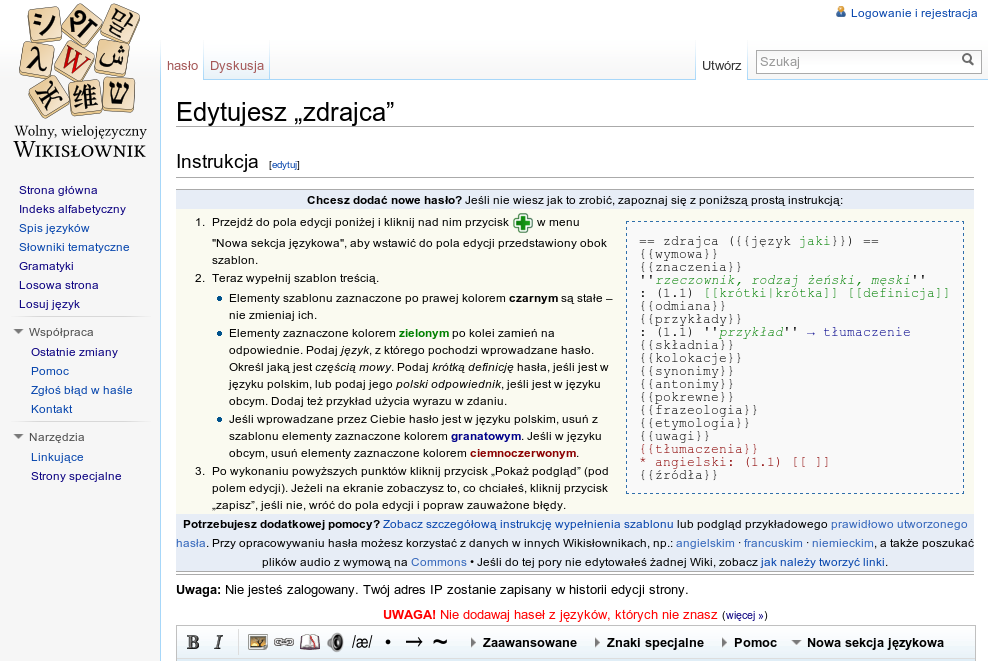
\includegraphics{plwikt-edit-non}}
	\caption{Próba stworzenia nowego hasła w~polskim Wikisłowniku}
	\label{fig:plnew}
\end{illustration}

Jak widać na zrzucie ekranu, sama instrukcja tworzenia nowego hasła jest na tyle skomplikowana, że może zniechęcić do edycji nowego redaktora. Wymagane jest skopiowanie podanego kodu i~pieczołowite podmienianie poszczególnych jego elementów. Niestety tylko w~bardzo ograniczonym stopniu uwzględniane jest, że niektóre języki mają zdecydowanie inną strukturę niż przykładowa. Osoba chcąca dodać do Wikisłownika nowy znak chiński będzie musiała nie tylko zapoznać się z~regułami dla tej specyficznej odmiany haseł, ale też prawdopodobnie skopiować kod istniejącego hasła z~tej kategorii. O~wiele lepsza byłaby sytuacja, w~której po wyborze języka edytujący otrzymuje odpowiedni szkielet hasła, który będzie mógł uzupełnić standardowym formularzem, bez potrzeby wybierania fragmentów, które należy zmienić lub usunąć.

Oparcie projektów Wikimedia na systemie MediaWiki i~wikikodzie powoduje tego typu problemy oczywiście nie tylko w~Wikisłowniku. Także w~Wikipedii komplikacje techniczne są dużą barierą dla nowych użytkowników, najczęściej przyzwyczajonych do narzędzi typu WYSIWYG (\emph{What You See Is What You Get}) takich jak Microsoft Word. W~badaniach przeprowadzonych w~2009~roku czytelnikom wszystkich wersji językowych Wikipedii zadano pytanie o~powody nieuczestniczenia w~pracach edycyjnych. 25,18\% spośród 21~492~ankietowanych odpowiedziało \emph{nie wiem, jak}; 12,49\% stwierdziło, że zbyt słabo zna używane technologie; natomiast 24,43\% wskazało, że obawiałoby się popełnienia błędu i~,,wpadnięcia w~kłopoty'' z~tego powodu (najczęściej wymienianym powodem było \emph{myślę, że nie mam wystarczającej wiedzy, którą mogę się podzielić} --- 51,98\%)~\cite{wiki:survey}. Wynika z~tego, że aż jedna czwarta czytelników, którzy wypełnili ankietę, to potencjalni redaktorzy, którzy nie angażują się w~tworzenie encyklopedii ze względu na uwarunkowania techniczne. Brak podobnych badań przeprowadzanych na użytkownikach Wikisłownika, można jednak przypuszczać, że kształtują się one podobnie. Dodatkowym czynnikiem jest specjalizacja projektu --- w~pracach przy słowniku w~dużej części uczestniczą lingwiści, którzy nie muszą biegle posługiwać się platformą MediaWiki.

W~przypadku Wikipedii od dawna podejmowane są wysiłki w~kierunku poprawienia obsługi technicznej serwisu. Istnieje np. alternatywny edytor haseł \emph{wikEd} dostępny dla każdego użytkownika po wybraniu w~preferencjach, w~ograniczonym zakresie wspomagający redagowanie haseł~\cite{wiki:wiked}. Prawdopodobnie jednak edytor WYSIWYG wspólny dla przedsięwzięć Fundacji Wikimedia nie powstanie w~przewidywalnej przyszłości. Z~tego powodu korzystne jest usprawnianie poszczególnych projektów z~uwzględnieniem ich cech charakterystycznych. Jednym z~celów opisywanej aplikacji jest zwiększenie komfortu korzystania z~formularza wprowadzania haseł w~Wikisłowniku. Implementacja tego projektu została omówiona w~podrozdziale~\ref{sec:impl-form}.

Drugą znaczącą wadą Wikisłownika jest wynikająca z~wielojęzyczności ogromna redundancja, powodująca spore problemy dla czytelnika. Każda wersja językowa stanowi odrębną całość. Choć słowników internetowych nierzadko używają poligloci, którym może być obojętne, w~jakim języku zostaną zaprezentowane informacje, struktura Wikisłownika nie pozwala im wykorzystać swoich umiejętności. Specjalistyczne hasła mogą być dostępne np. wyłącznie w~jednej wersji językowej --- przeszukiwanie poszczególnych edycji to marnotrawienie czasu, dlatego często najlepszym rozwiązaniem bywa po prostu użycie wyszukiwarki, np. Google. Informacje w~różnych językach pojawiają się niezależnie od siebie, bowiem znakomita większość redaktorów jest aktywna wyłącznie w~jednym projekcie. Przy tym zdarza się, że wprowadzający informacje wykonuje zupełnie niepotrzebną pracę, którą ktoś wykonał wcześniej w~innej wersji językowej, a~nawet w~tej samej wersji, lecz podczas tworzenia innego hasła, w~pewien sposób powiązanego z~obecnie edytowanym.

Ważną funkcję we wszystkich projektach Wikimedia pełnią boty, odpowiadające w~największych projektach za od~10 do 30\% wszystkich edycji haseł~\cite{bots}. W~polskim Wikisłowniku programy te przede wszystkim uzupełniają linki interwiki, ale także wykonują bardziej skomplikowane akcje: standaryzują układ podsekcji i~format linków, aktualizują indeksy i~inne listy słów oraz dodają polską wymowę~\cite{wikt:boty}~\cite{wikt:olafbot}. Część z~tych edycji jest wtórna i~spowodowana błędami popełnianymi przez początkujących redaktorów --- można by ich zatem uniknąć, usprawniając formularz edycji.

Automatyzacja edytora pozwala na sprawniejszą standaryzację i~użycie informacji wprowadzonych już do innych wersji językowych Wikisłownika. Bardzo pomocne okazuje się tu API MediaWiki~\cite{mw:api}. Ten interfejs programistyczny pozwala na sprawne pobieranie treści wybranych haseł z~dowolnego projektu Wikimedia w~celu dalszego przetwarzania. Zostało to wykorzystane podczas implementacji drugiej istotnej części aplikacji, a~następnie opisane w~podrozdziale~\ref{sec:impl-auto}.


\subsection{Różnice w~stosunku do Wikipedii}
\label{subs:wiki-wikt}
Po analizie uwidacznia się odmienny charakter Wikisłownika w~stosunku do Wikipedii, która była pierwszym projektem Fundacji i~dziś jest jej sztandarowym przedsięwzięciem. W~tabeli~\ref{tab:wiki-wikt} zostały ujęte najważniejsze różnice między witrynami w~aspekcie technicznym.
\begin{table}[h]
\begin{center}
	\begin{tabularx}{\textwidth}{ XX }
		\toprule \textbf{Wikipedia} & \textbf{Wikisłownik} \\
		\toprule Struktura hasła różnorodna
			& Bardzo ściśle określona struktura hasła \\
		\midrule Przede wszystkim ciągły tekst
			& Listy, wypunktowania \\
		\midrule Umiarkowana liczba szablonów używanych w~hasłach w~stosunku do pozostałej treści
			& Bardzo duży udział szablonów w~treści hasła \\
		\midrule Duże różnice pomiędzy wersjami językowymi
			& Małe różnice pomiędzy wersjami językowymi \\
		\midrule Linki interwiki łączą informacje o~tym samym obiekcie w~różnych językach
			& Linki interwiki łączą informacje o~tym samym słowie występującym w~wielu językach, objaśnione w~różnych językach \\
		\midrule Nagłówki dzielą artykuł na sekcje o~dowolnej semantyce
			& Nagłówki dzielą artykuł na sekcje odpowiadające poszczególnym językom \\
		\bottomrule
	\end{tabularx}
\caption
	[Porównanie Wikipedii i~Wikisłownika --- aspekty techniczne]
	{Porównanie Wikipedii i~Wikisłownika --- aspekty techniczne. Zob. też tabelę \ref{tab:wiki-wikt2}}
\label{tab:wiki-wikt}
\end{center}
\end{table}

To wszystko powoduje, że usprawnienie edycji w~Wikisłowniku jest o~wiele łatwiejsze niż w~Wikipedii, której bardzo złożona struktura w~praktyce uniemożliwia dziś kompleksową przebudowę procesu redakcji. Ściśle określona struktura to ogromna zaleta projektu. Co ciekawe --- nie jest ona charakterystyczna dla wszystkich jego wersji językowych. Po wykonaniu części prac włożonych w~implementację okazało się, że polski Wikisłownik jest pod tym względem wyjątkowo dobrze zorganizowany. Wprawdzie wszystkie większe edycje zachowują standardowy podział na sekcje językowe, jednak owe sekcje niekiedy przybierają dość oryginalne postaci. Po dokładniejszych badanich można stwierdzić, że polski Wikisłownik jest wyjątkowo jednolity, co ma niebagatelne znaczenie zarówno dla czytelnika, jak i~dla edytora. W~kolejnym rozdziale zanalizowano m.in. specyfikę Wikisłownika, jeśli skupić się na aspektach społecznościowych. Jak się okaże, także te elementy powinny mieć pozytywny wpływ na możliwość wprowadzenia usprawnień.
